\chapter{Analyse et conception}
Ce chapitre présente l'étude de l'existant avec une analyse et description des besoins, ainsi que les étapes établies pour réaliser le projet.
\newpage

\section{Étude et analyse des besoins}
\subsection{Étude de l'existant}
La gestion de l'emplois  du temps est une tâche trés importante que ça soit pour les étudiants ou bien les professeurs, plusieurs parmis les étudiants içi à l'ENSIAS trouvent que parfois l'emplois du temps n'est pas publié tôt, mais le fait de contacter chaque professeur et arriver à un compromis qui satisfait tout le monde, prend énormement du temps de chef de fillère. D'où vient le besoin à une application web qui automatise ce long processus.
\subsection{Capture des besoins}
Le projet qui nous a été accordé consiste à répondre aux besoins suivants:
\subsubsection{Besoins fonctionnels}
\begin{itemize}
    \item La possibilité pour les profs de choisir les heures pendant les quelles ils seront disponibles.
    \item Gestion des utilisateurs.
    \item Génération un emplois du temps en se basant sur la disponibilté des professeurs et des salles.
    \item Génération un fichier qui peut être téléchargé est inséré dans Google Calendar pour rappeller un prof qu'il a un cours ou un TD à une heure donnée.
\end{itemize}

\subsubsection{Besoins non-fonctionnels}
\begin{itemize}
  \item maintenabilité: L'application doit être facile à maintenir, de manière cohérente et à moindre coût, en état de fonctionnement, pour laisser la possibilité à d'autres ingénieurs de modifier l'appication et l'adapter selon le besoin d'une autre école.
  \item  Efficacité: L'application doit marcher correctement sans erreurs.
  \item  Simplicité : L'interface doit être simple et facile à utiliser.
  \item Sécurité : L'application contient des données de l'école, et donc il faut les protéger en procédant par des logins et mots de passe.
  \item Disponibilté : L'application doit être tout le temps à la disposition de l'utilisateur.
   
\end{itemize}  

\section{Conception de la solution}

\subsection{Diagramme de classes}
 \begin{figure}[!htb]
      \centering
        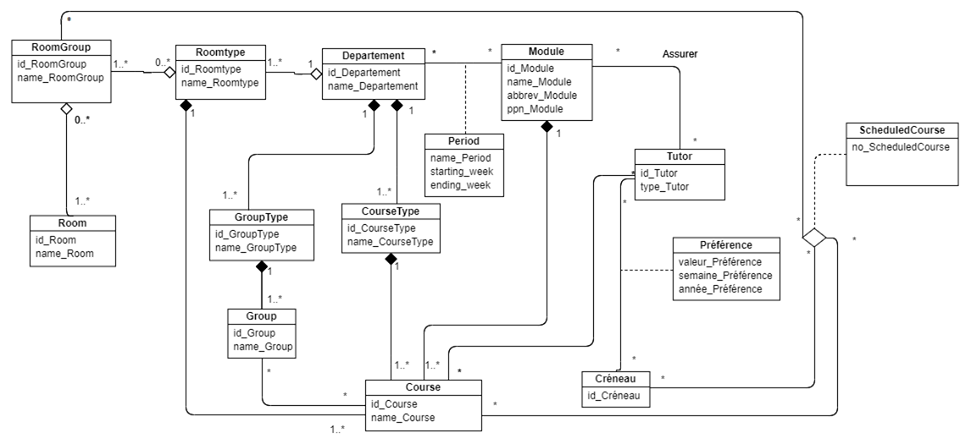
\includegraphics[width=17cm,height=21cm]{img/ClassDiagramm.png}
        \caption{Scénario :Diagramme de classe. }
    \end{figure}
\newpage

\\
\subsection{Diagramme de cas d'utilisation}
 \begin{figure}[!htb]
      \centering
        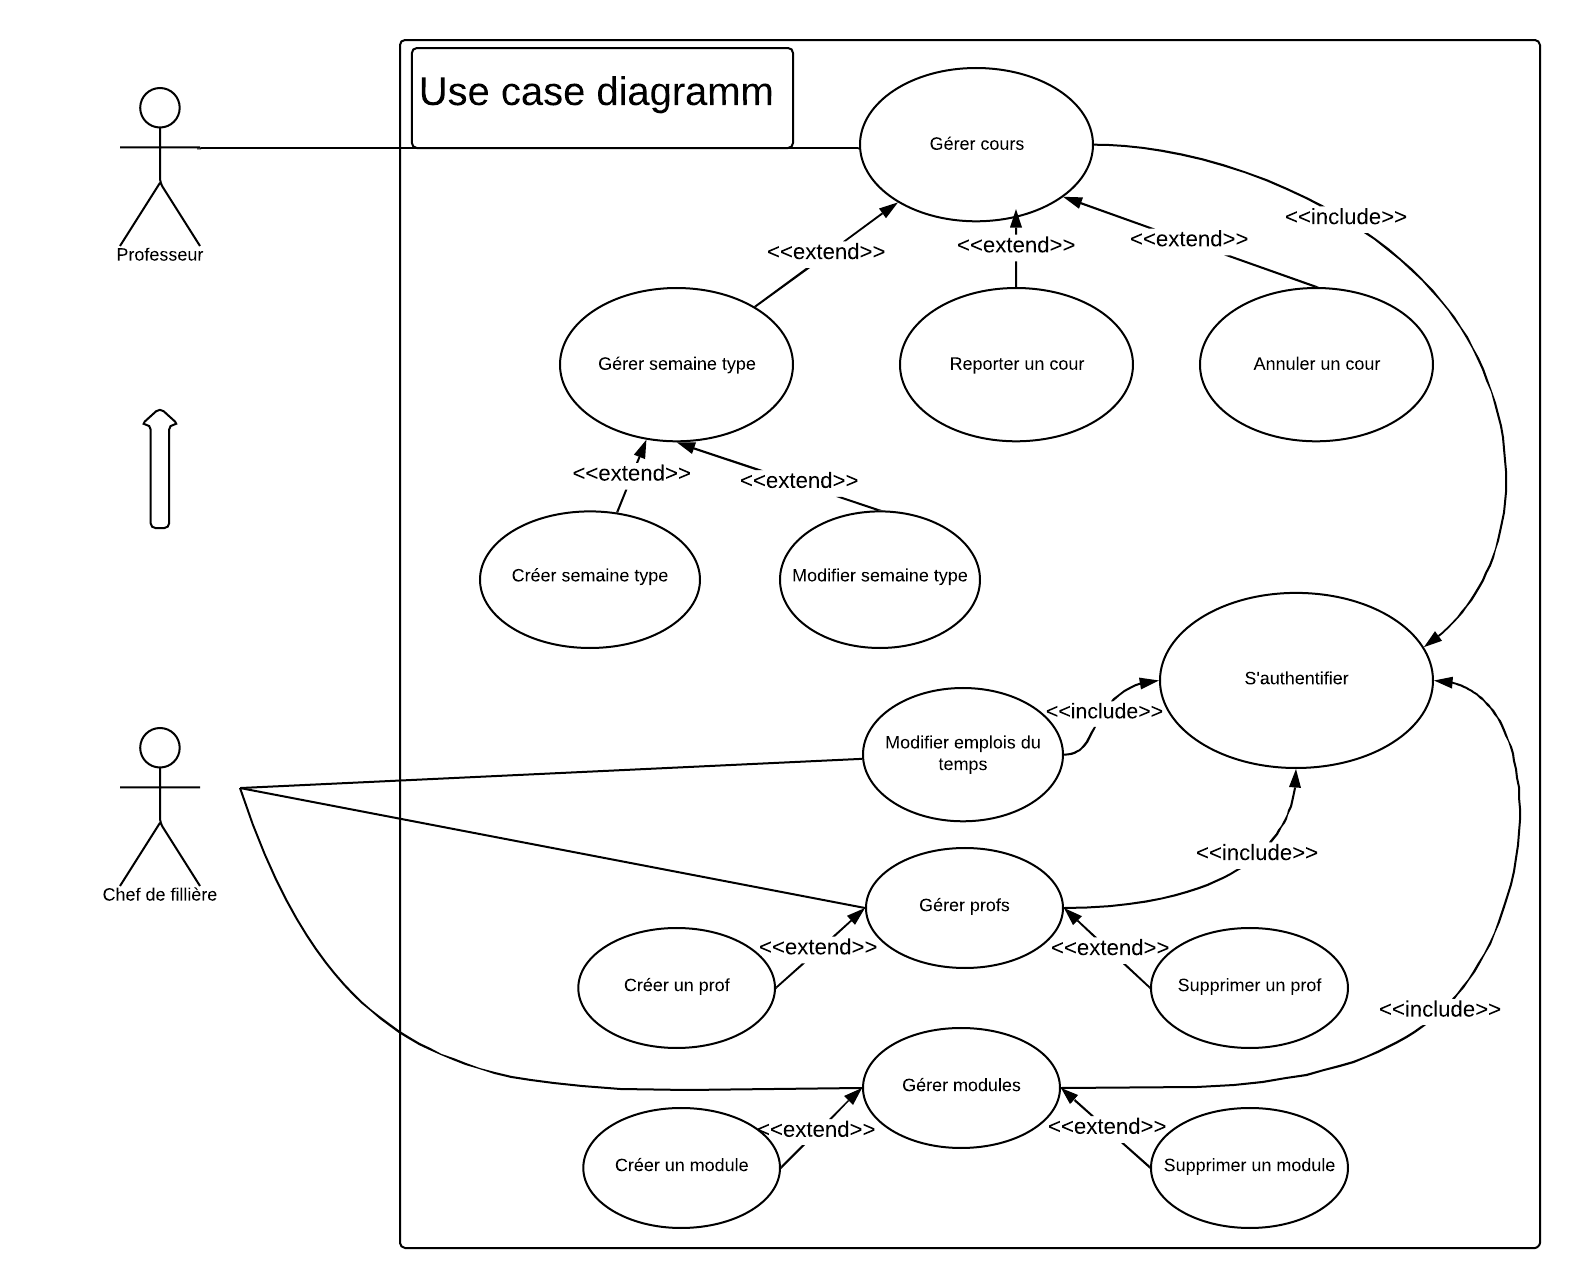
\includegraphics[width=15cm,height=18cm]{img/UseCase.png}
        \caption{Diagramme de cas d'utilisation. }
    \end{figure}
\newpage 

\subsection{Diagrammes de séquence}
Les diagrammes suivants représentent quelque scénarios possibles pour l'utilisateur de l'application que ça soit le prof ou le chef de fillière:
\subsubsection*{S'authentifier}
L'utilisateur saisi sont login et mot de passe, en cas d'erreur l'application lui demande de retaper les informations demandées.
 \begin{figure}[!htb]
      \centering
        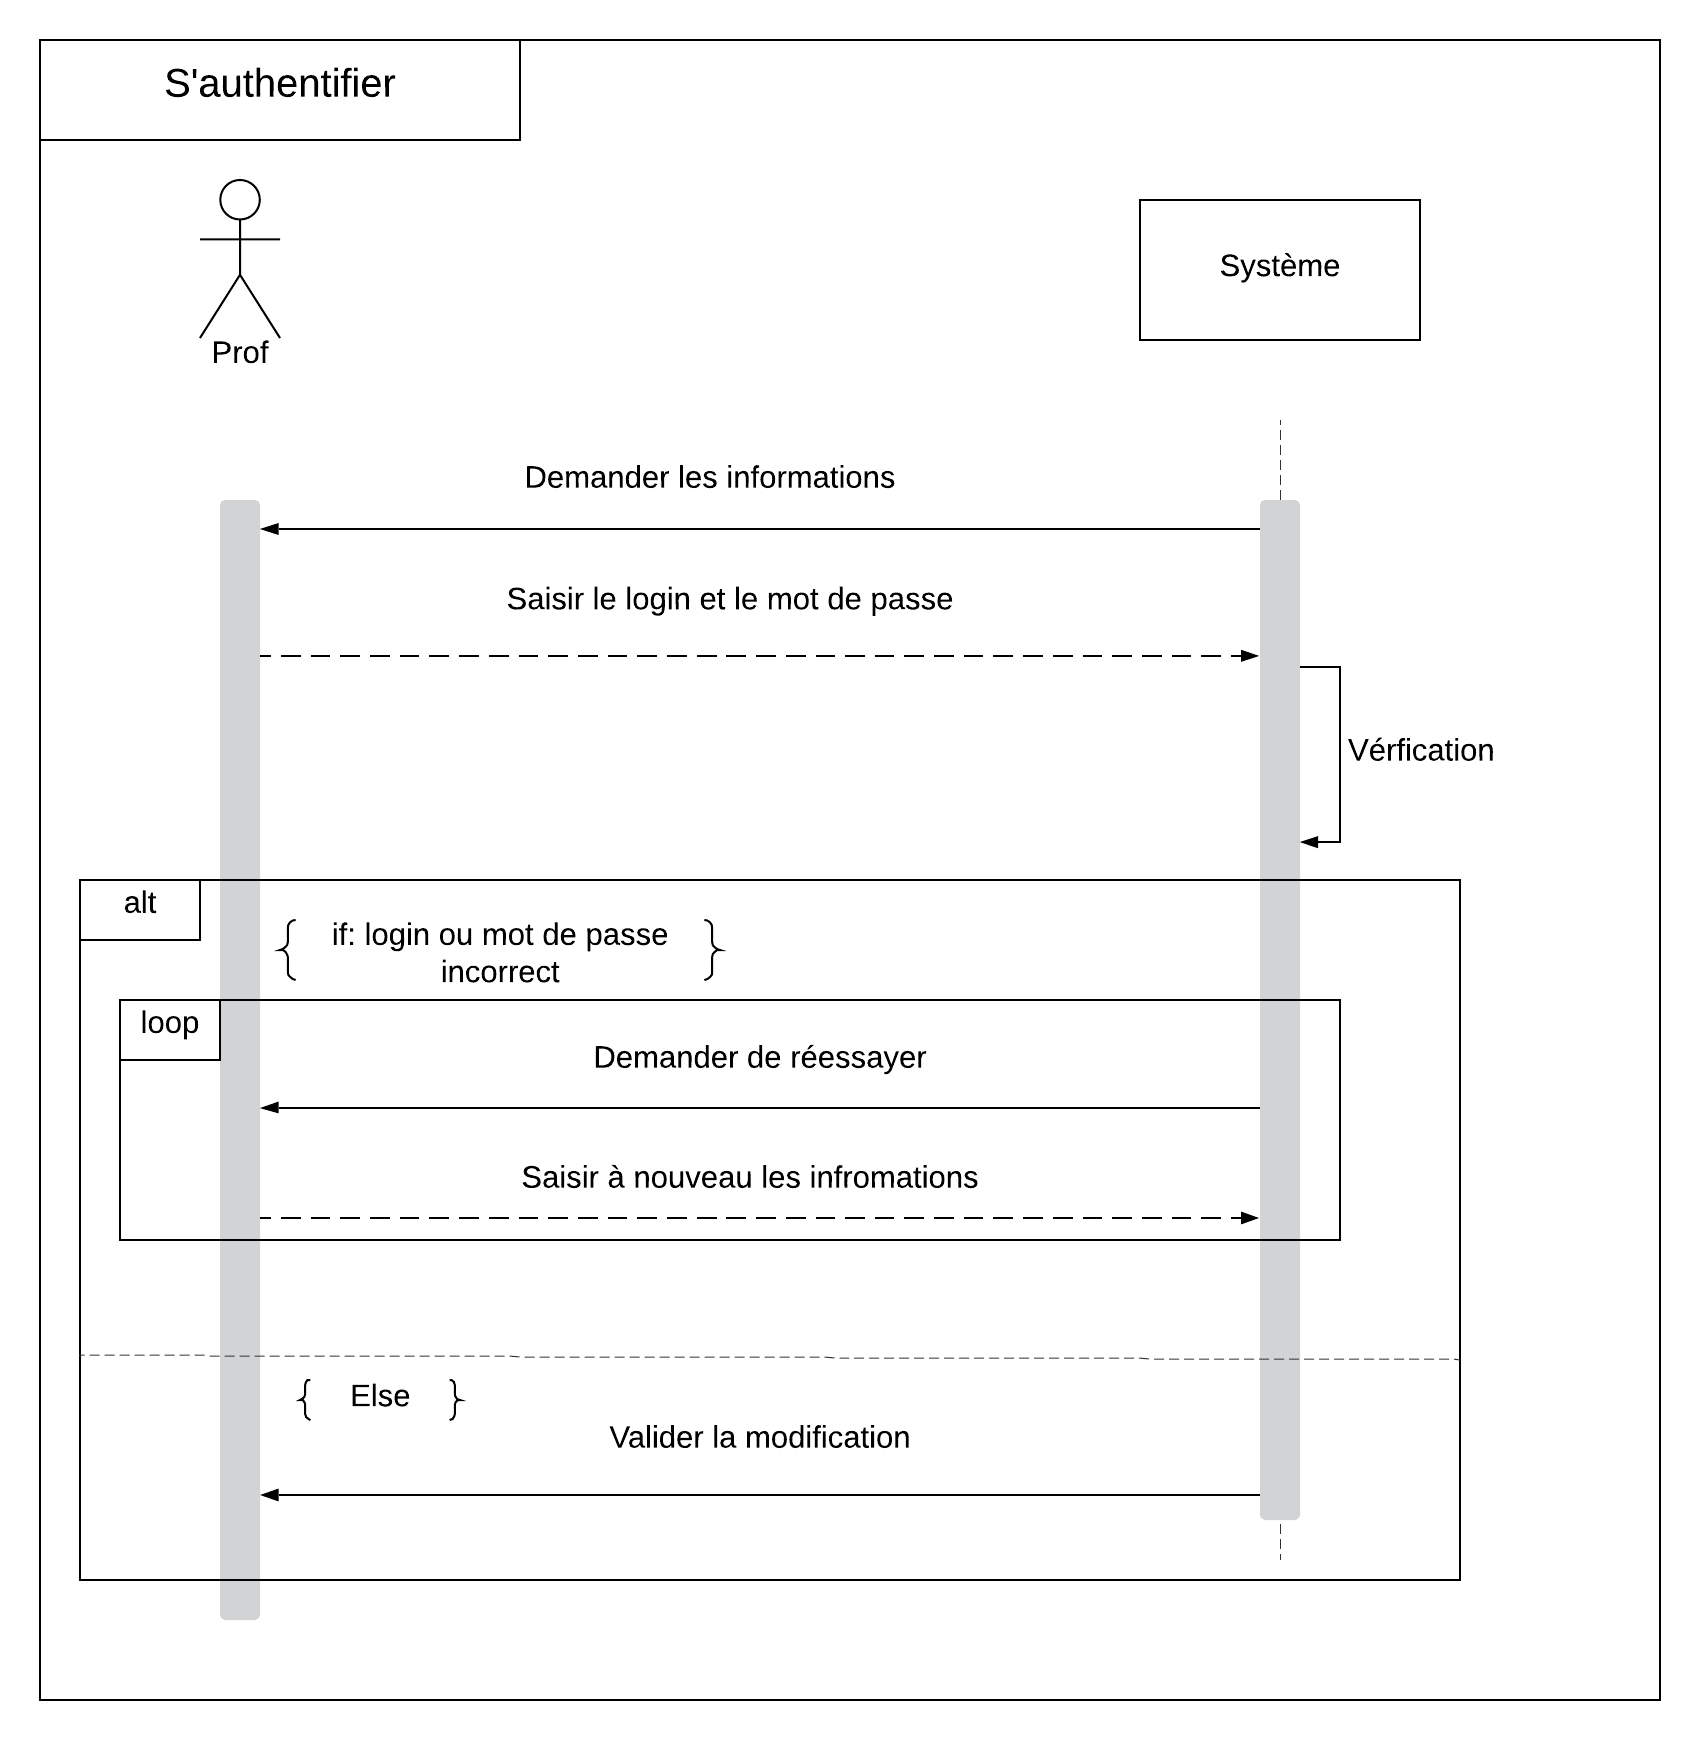
\includegraphics[width=15cm,height=16cm]{img/S'authentifier.png}
        \caption{Scénario d'authentification. }
    \end{figure}
    
\newpage

\subsubsection*{Créer semaine type}
Le prof sélectionne les heures pendant les quelles il est disponible.
 \begin{figure}[!htb]
      \centering
        \includegraphics[width=15cm,height=18cm]{img/CréerSemType.png}
        \caption{Scénario :Créer Semaine Type. }
    \end{figure}
\newpage
\subsubsection*{Modifier semaine type}
Le prof modifie les heures pendant les quelles il est disponible, en changeant ses préférences.
 \begin{figure}[!htb]
      \centering
        \includegraphics[width=15cm,height=18cm]{img/CréerSemType.png}
        \caption{Scénario :Modifier Semaine Type. }
    \end{figure}
 \newpage
 \subsubsection*{Reporter un cours}
Le prof peut reporter un cours, en précisant la date du rattrappage, mais s'il y a une contraine qui empêche d'avoir cette nouvelle séance, un message d'erreur est affiché.
 \begin{figure}[!htb]
      \centering
        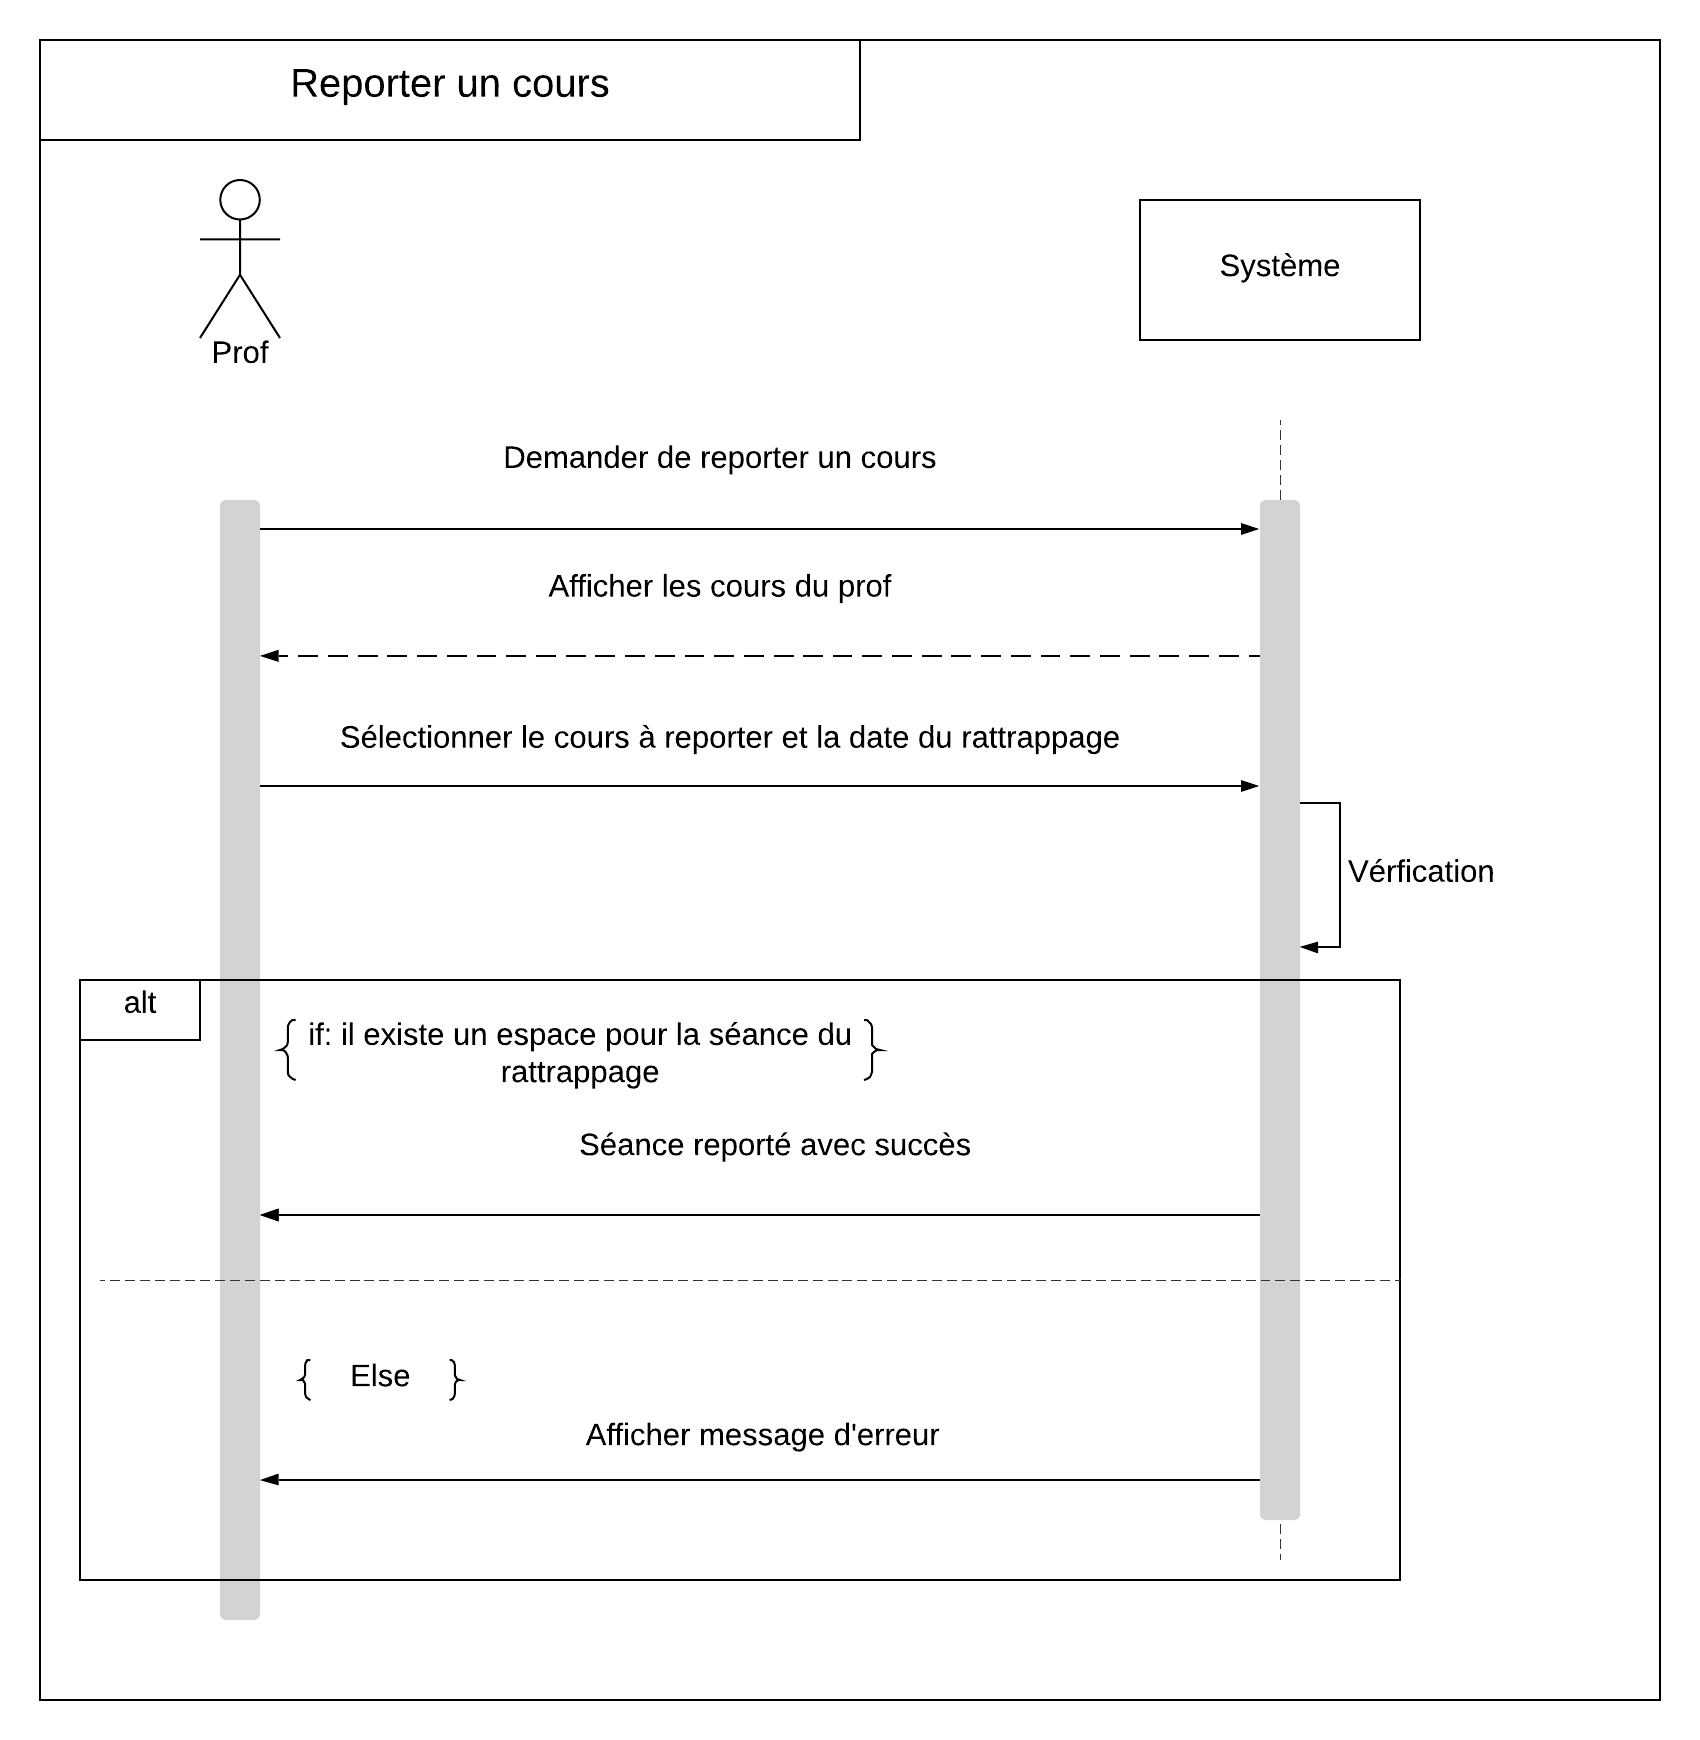
\includegraphics[width=15cm,height=18cm]{img/ReporterCours.png}
        \caption{Scénario :Reporter un cours. }
    \end{figure}   
\newpage
\subsubsection*{Annuler un cours}
Le prof peu annuler un cours.
 \begin{figure}[!htb]
      \centering
        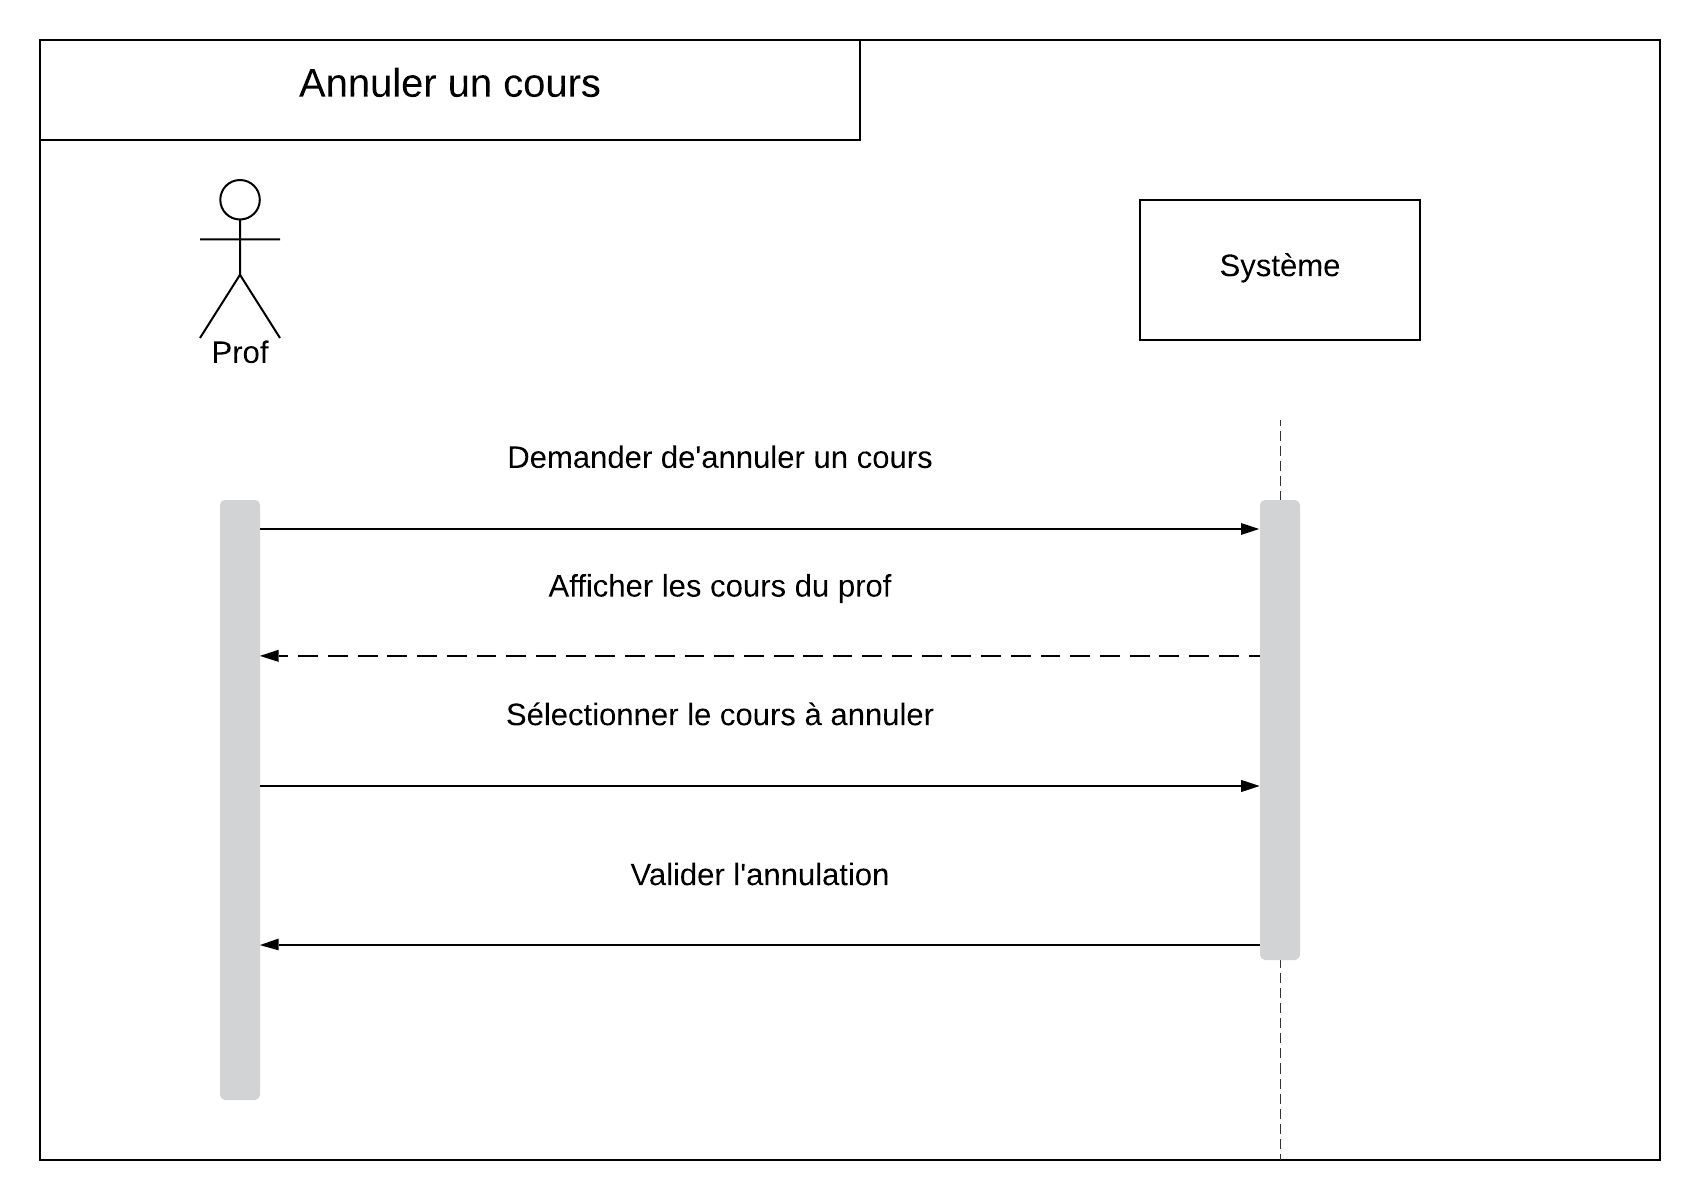
\includegraphics[width=15cm,height=18cm]{img/AnnulerCours.png}
        \caption{Scénario :Annuler un cours. }
    \end{figure}
\newpage
\subsubsection*{Créer prof}
Dans l'interface admin, le chef de fillière peut ajouter un nouveau prof, si un champ est vide, un message d'erreur est affiché.
 \begin{figure}[!htb]
      \centering
        \includegraphics[width=15cm,height=18cm]{img/CréerProf.png}
        \caption{Scénario :Créer un prof. }
    \end{figure}
\newpage
\subsubsection*{Summprimer un  prof}
Dans l'interface admin, le chef de fillière peut supprimer un prof.
 \begin{figure}[!htb]
      \centering
        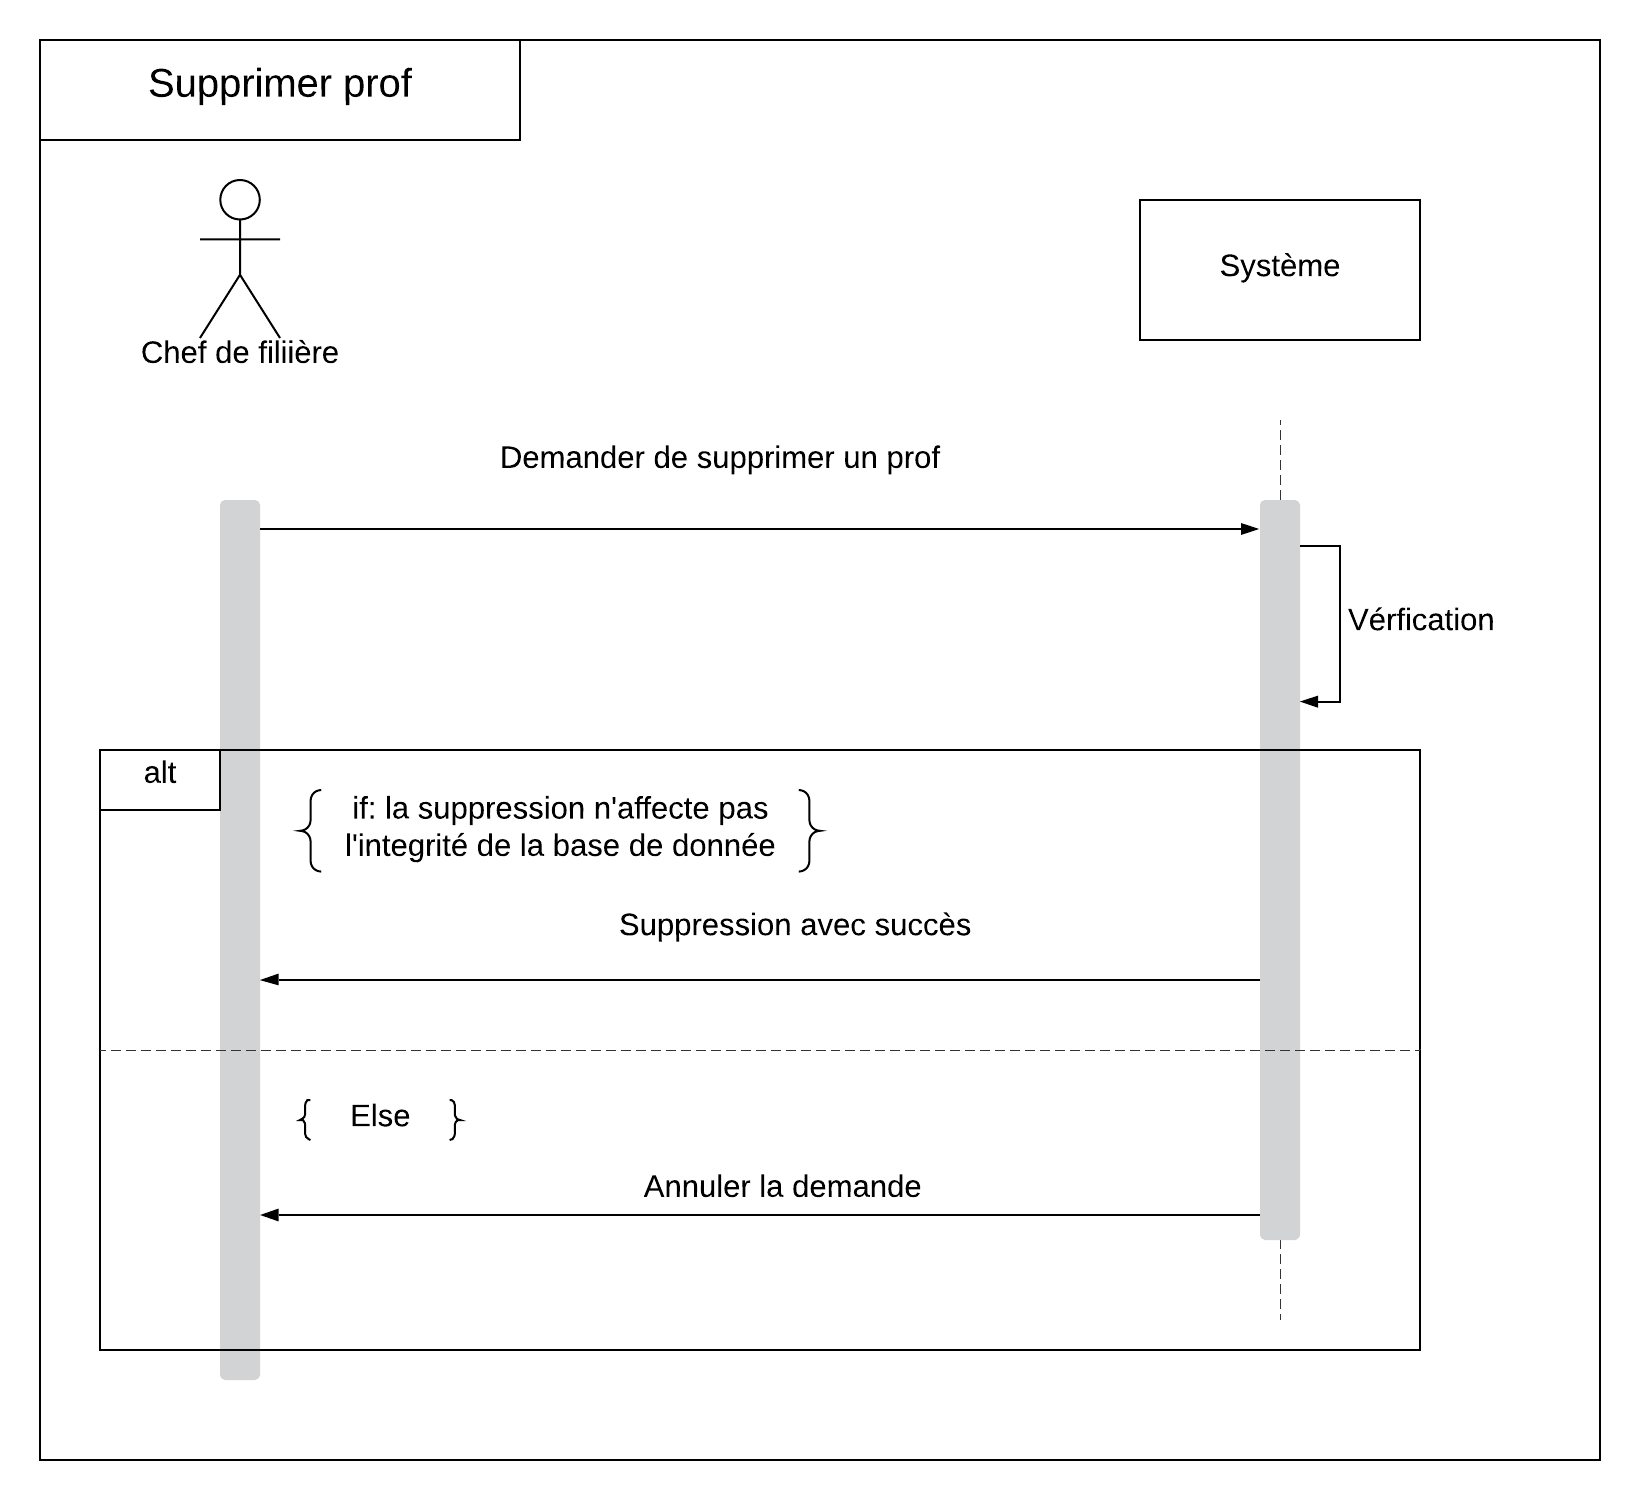
\includegraphics[width=15cm,height=18cm]{img/SupprimerProf.png}
        \caption{Scénario :Supprimer un prof. }
    \end{figure}
\newpage
\subsubsection*{Créer module}
Dans l'interface admin, le chef de fillière peut ajouter un nouveau module, si un champ est vide, un message d'erreur est affiché.
 \begin{figure}[!htb]
      \centering
        \includegraphics[width=15cm,height=18cm]{img/CréerModule.png}
        \caption{Scénario :Créer un module. }
    \end{figure}
\newpage
\subsubsection*{Summprimer un  module}
Dans l'interface admin, le chef de fillière peut supprimer un module.
 \begin{figure}[!htb]
      \centering
        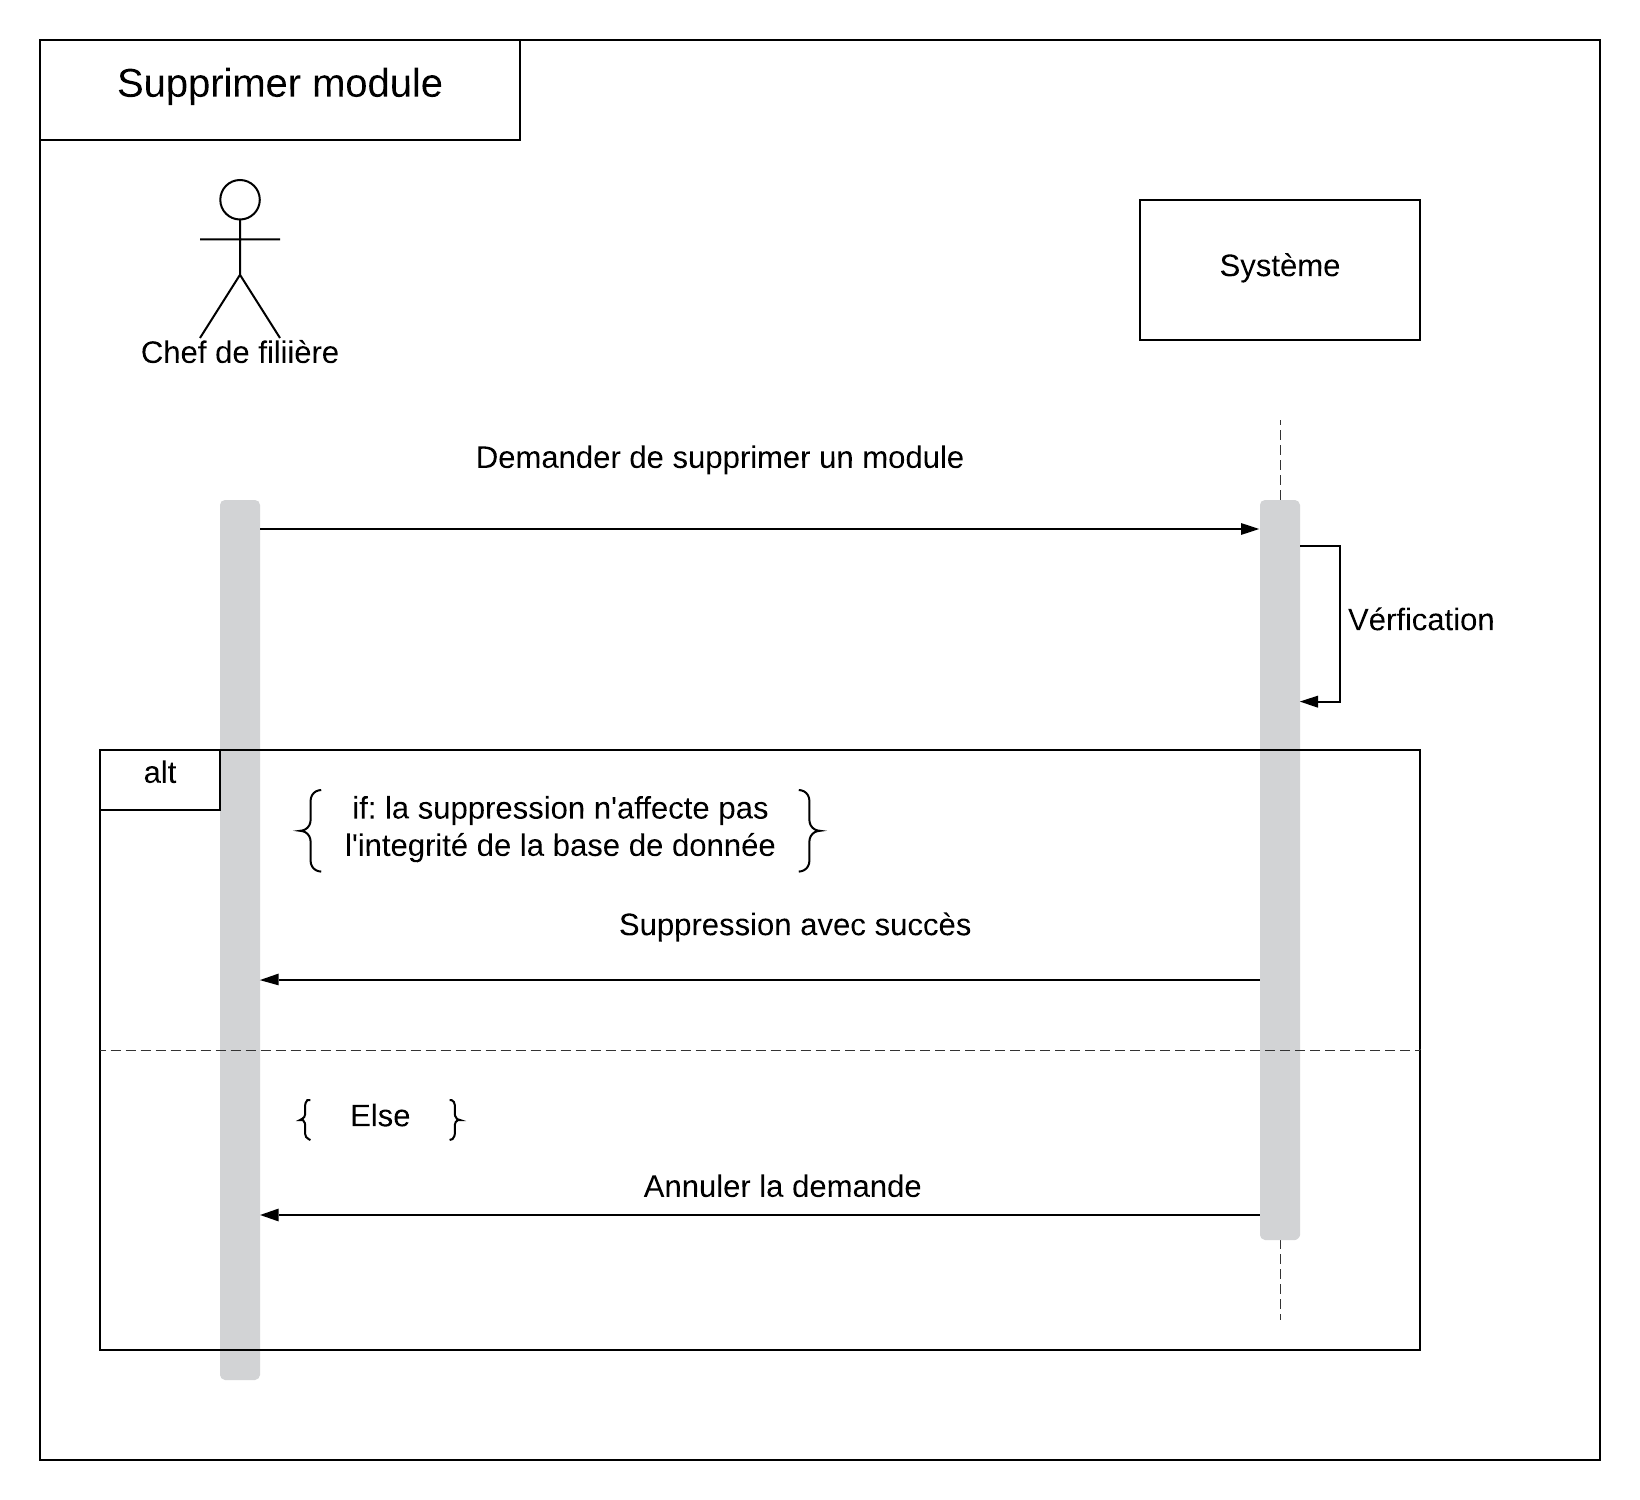
\includegraphics[width=15cm,height=18cm]{img/SupprimerModule.png}
        \caption{Scénario :Supprimer un module.}
    \end{figure}









